% ----------------------------------------------------------------------- %
% Arquivo: anexo.tex
% ----------------------------------------------------------------------- %

\chapter{}

\begin{figure}[htb]
    \centering  % figura centralizada
    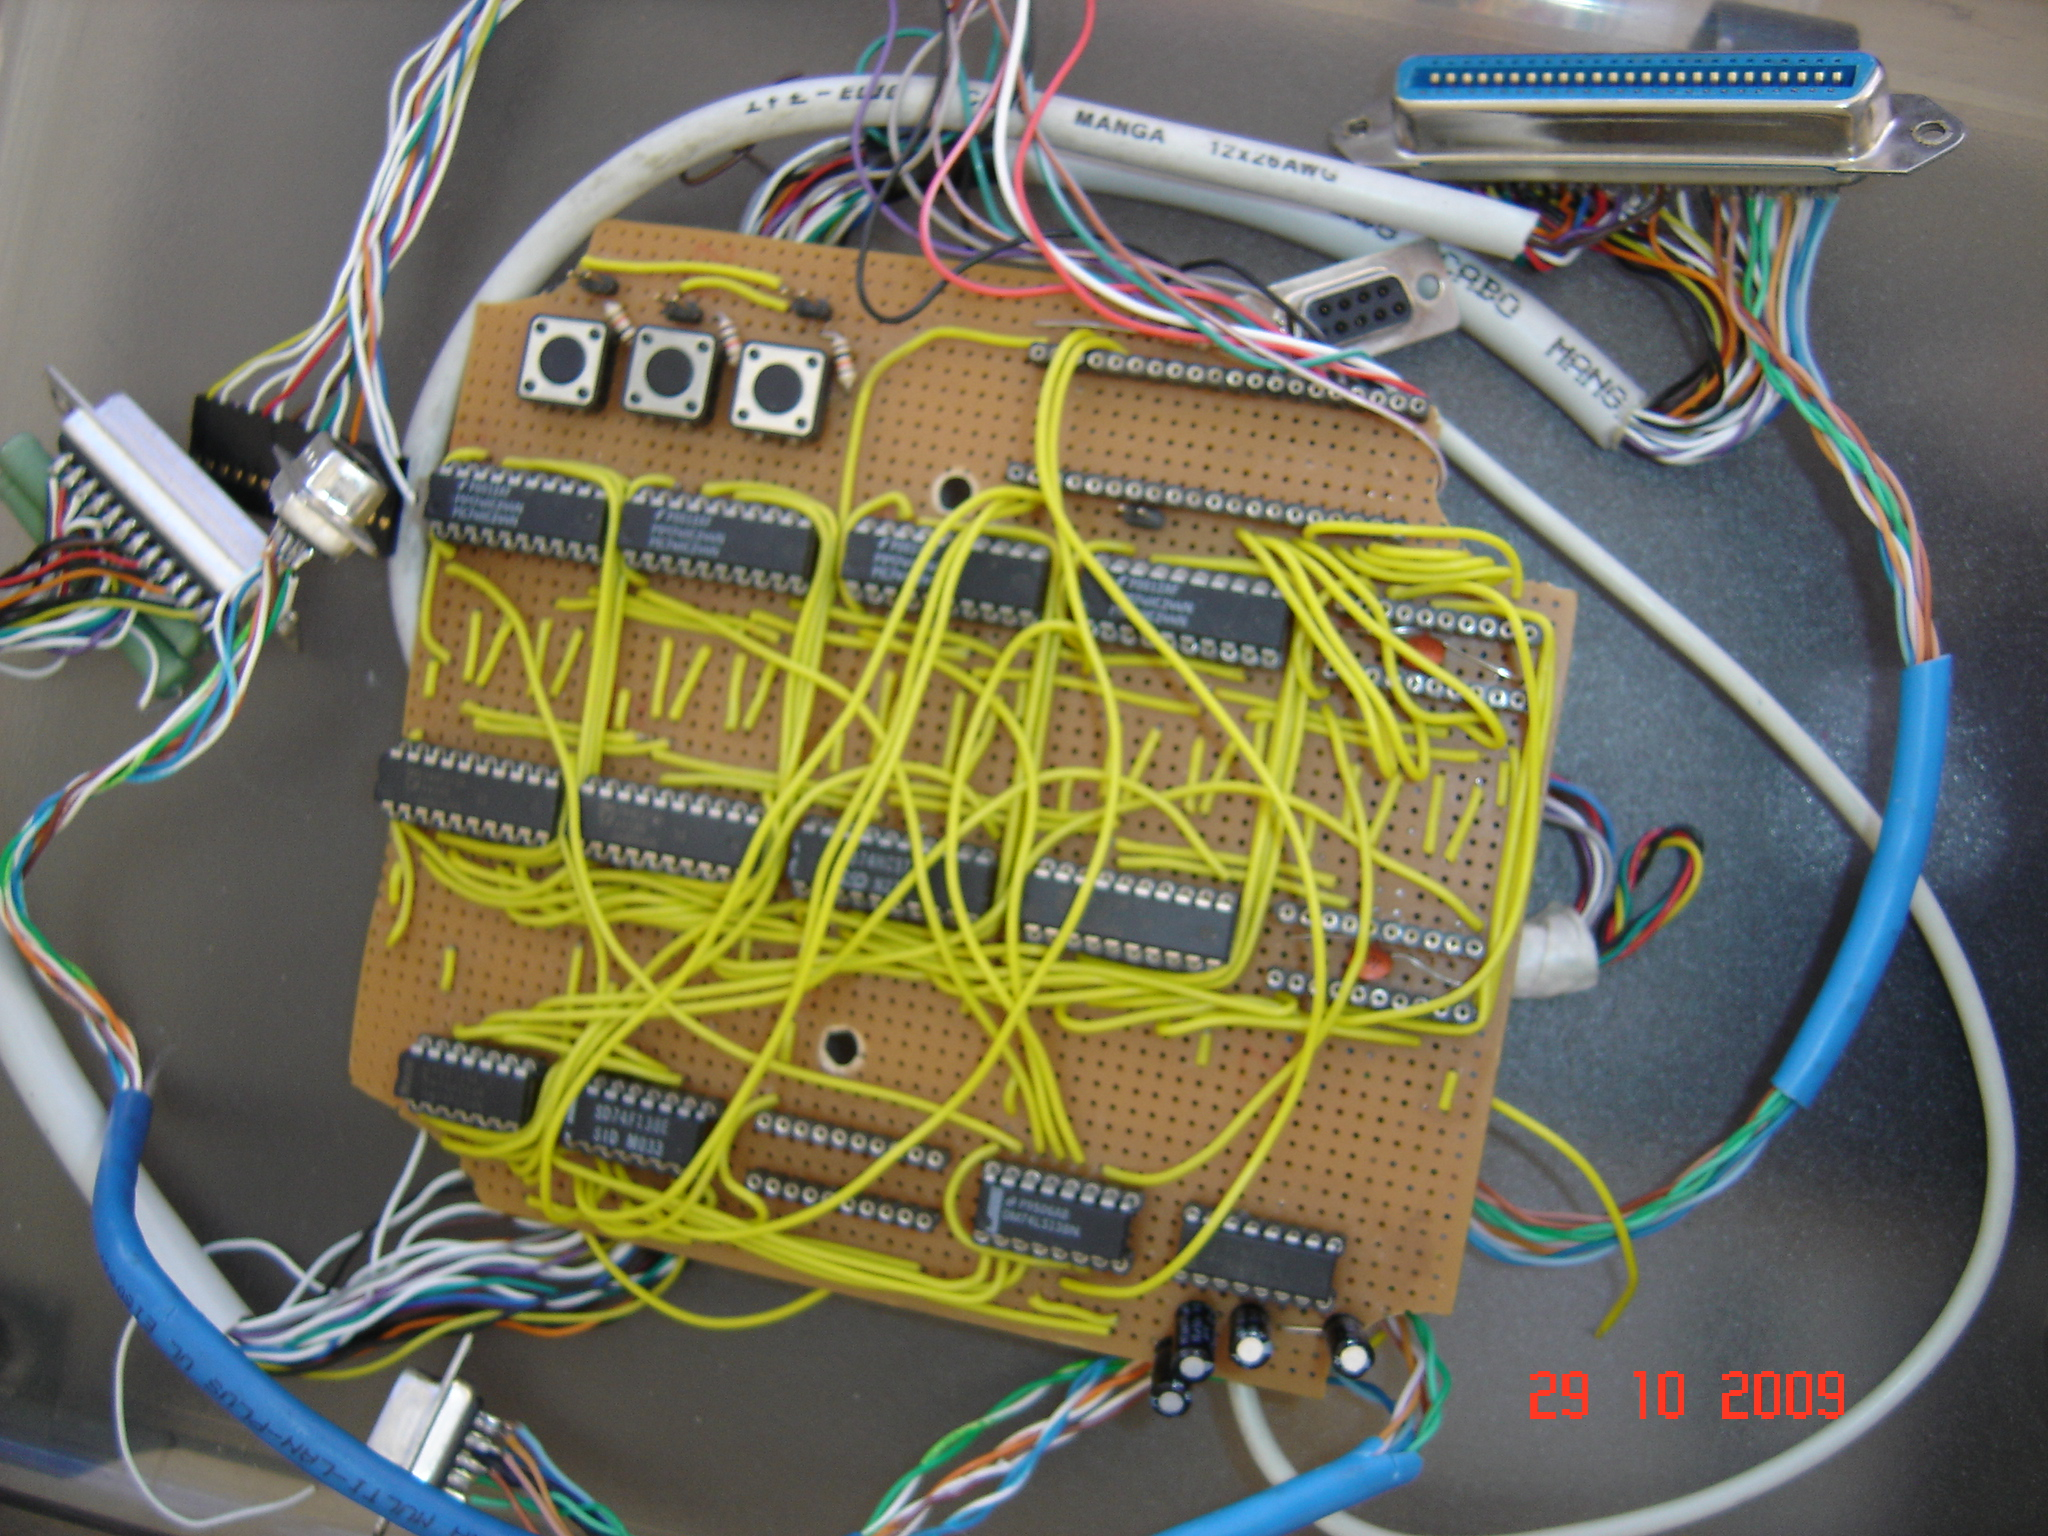
\includegraphics[scale=0.2]{anexo/a1.JPG}
    \caption{\it Foto da placa prot�tipo - frente}
\end{figure}

\begin{figure}[htb]
    \centering  % figura centralizada
    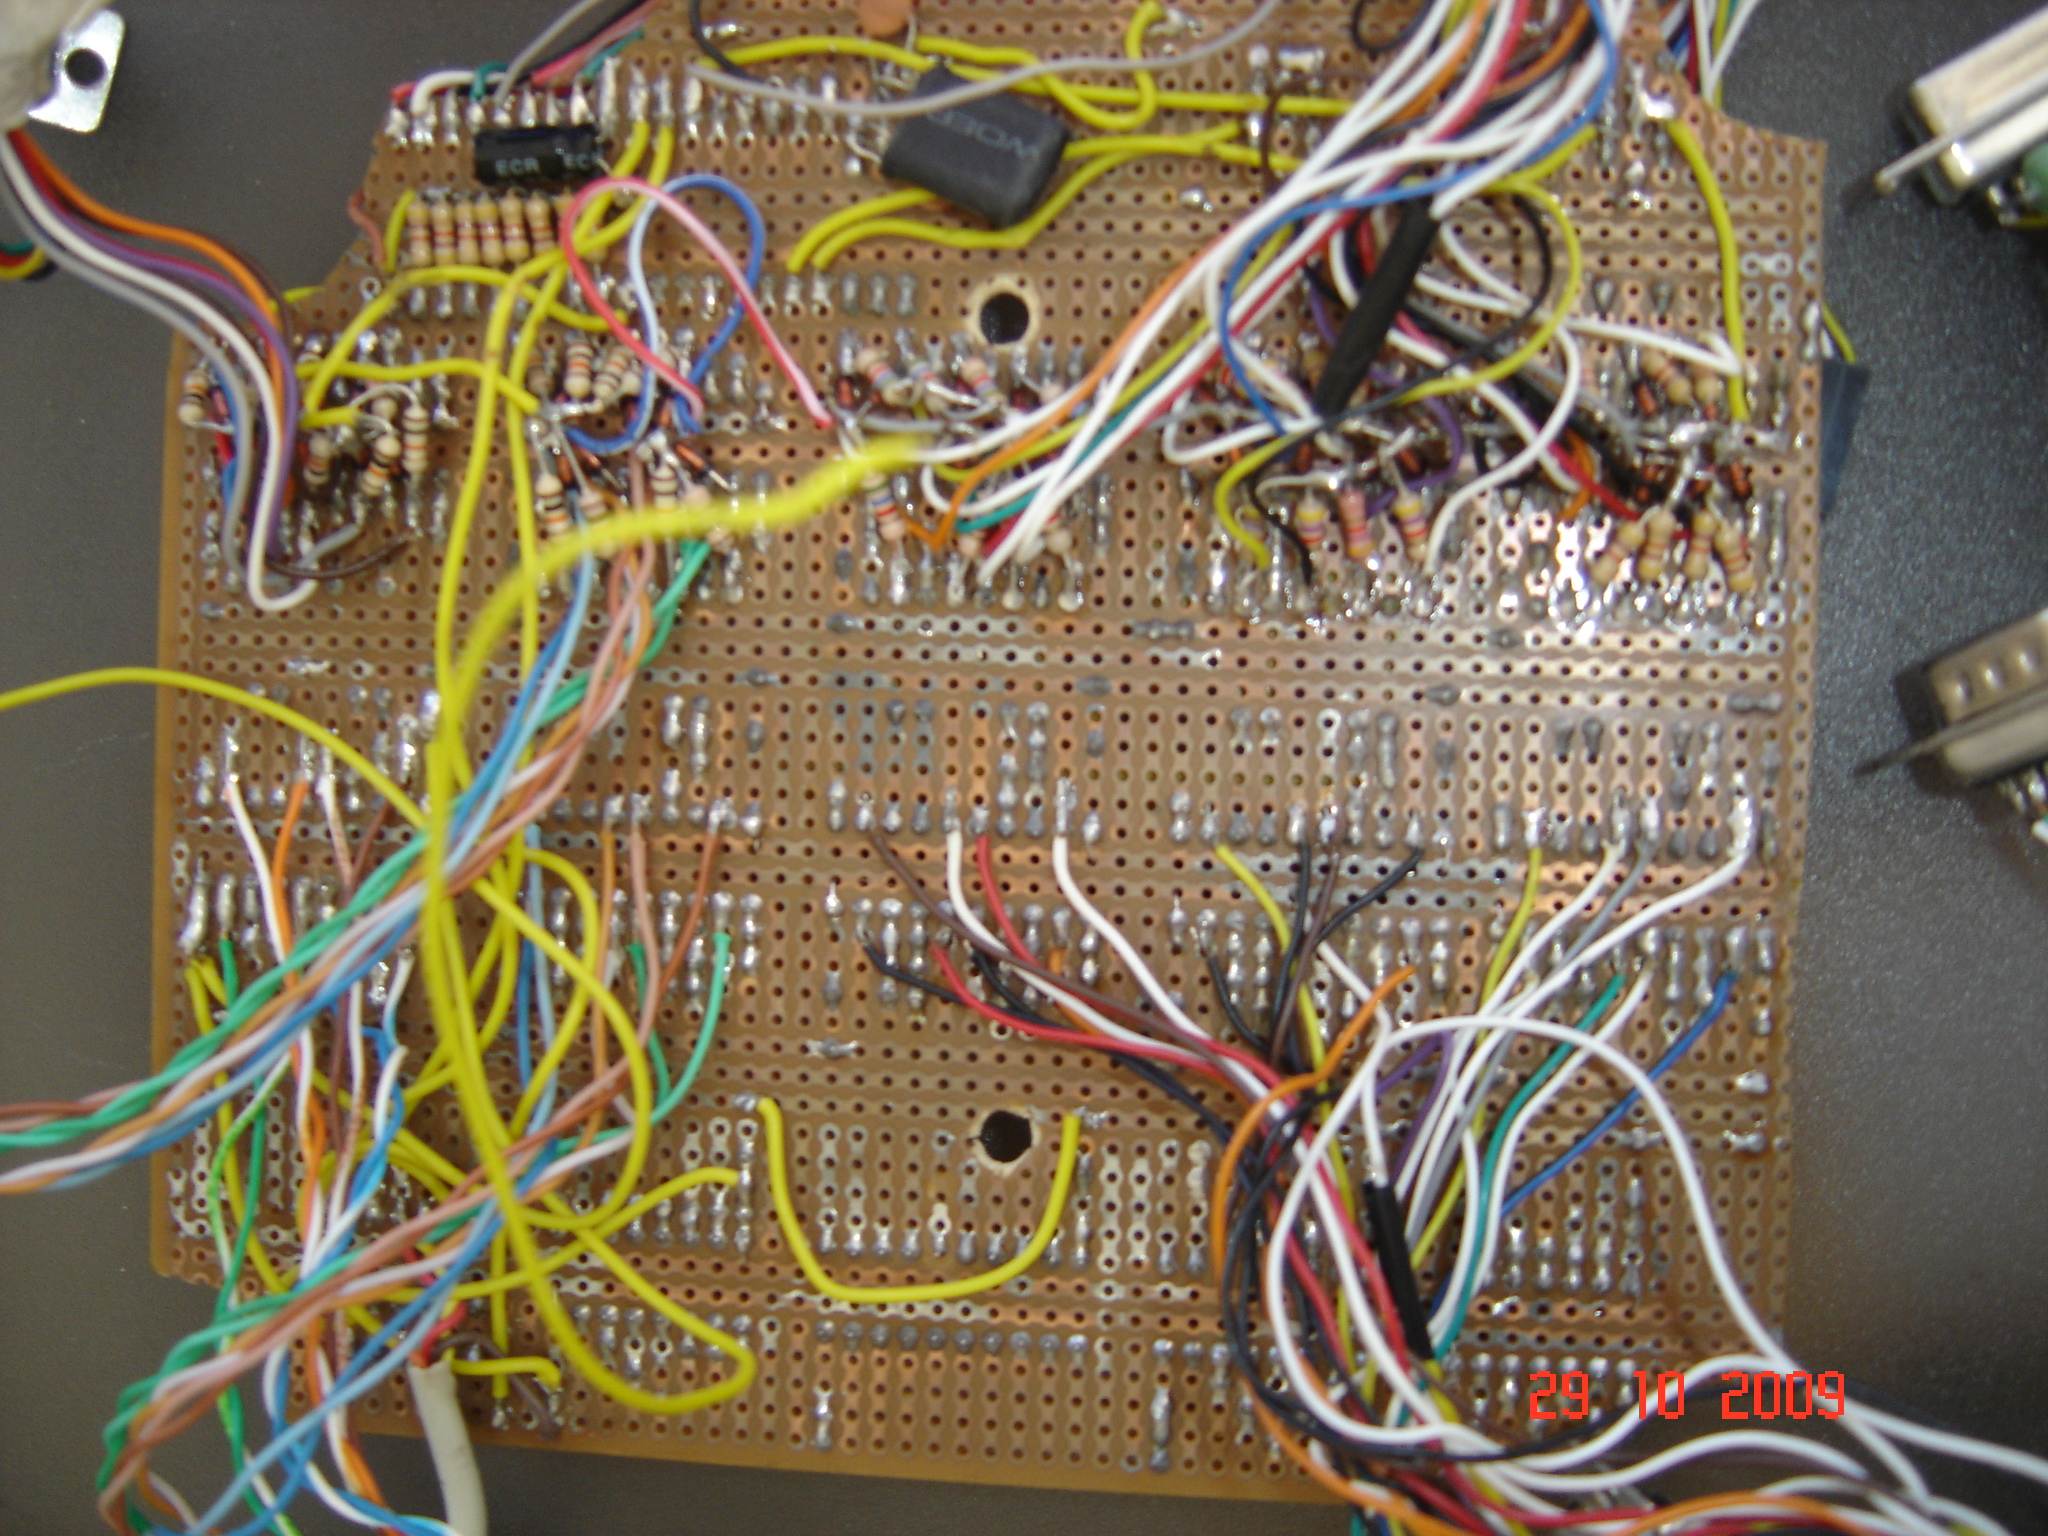
\includegraphics[scale=0.2]{anexo/a2.JPG}
    \caption{\it Foto da placa prot�tipo - verso}
\end{figure}

\begin{figure}[htb]
    \centering  % figura centralizada
    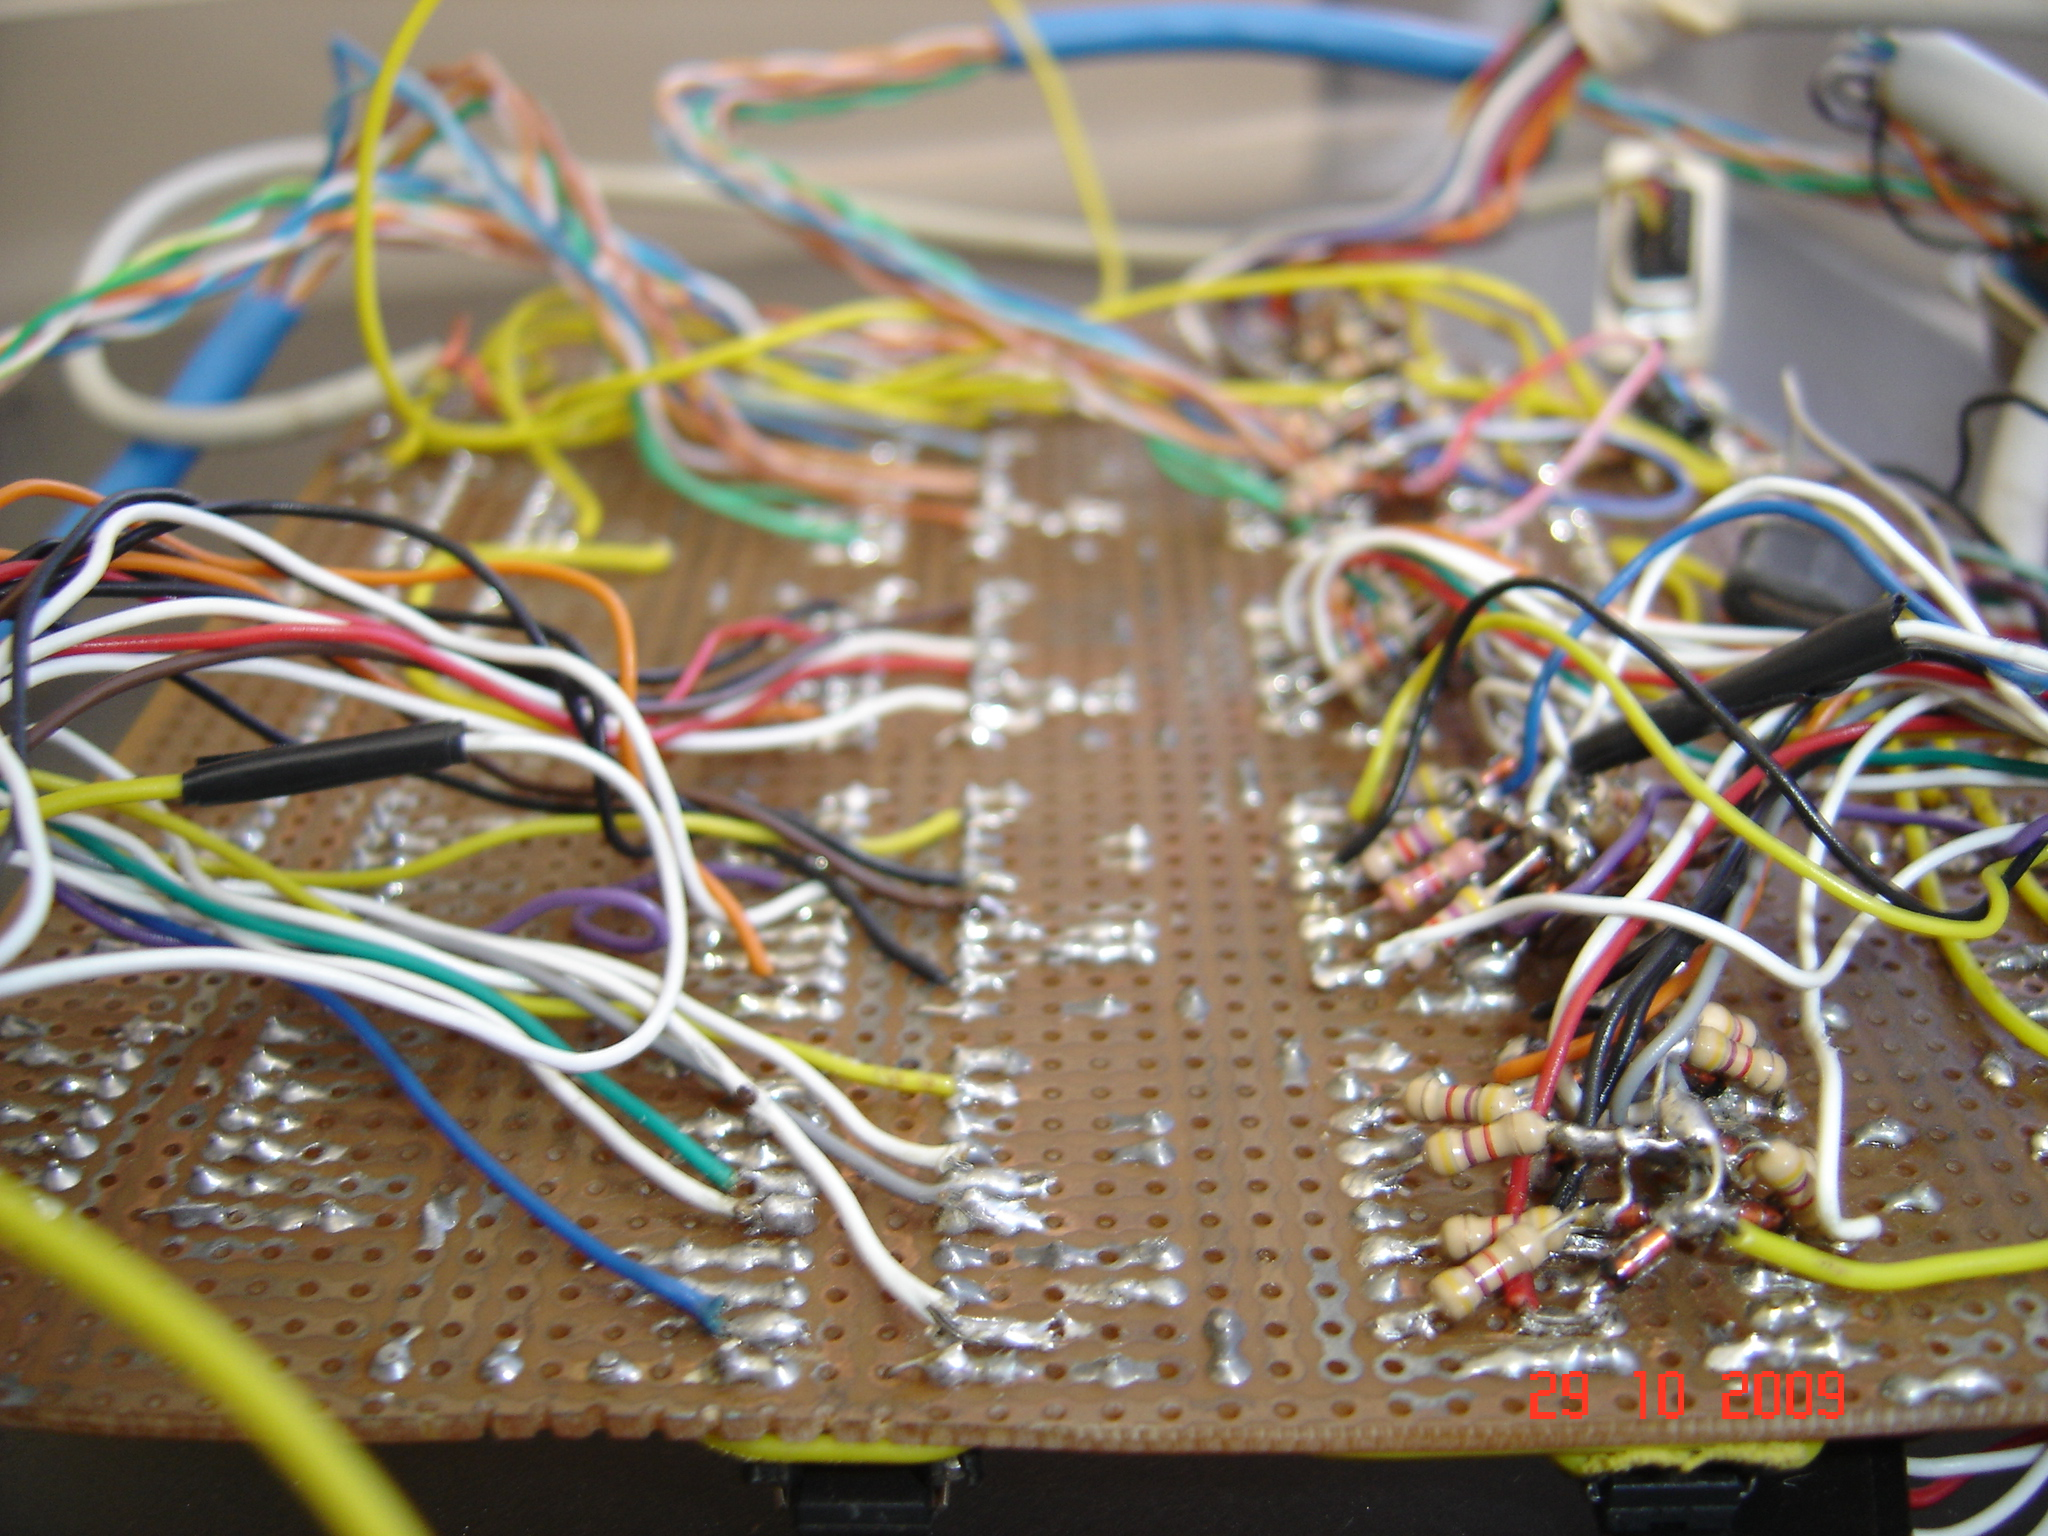
\includegraphics[scale=0.2]{anexo/a3.JPG}
    \caption{\it Foto da placa prot�tipo - diagonal}
\end{figure}

\chapter{}

\begin{figure}[htb]
    \centering  % figura centralizada
    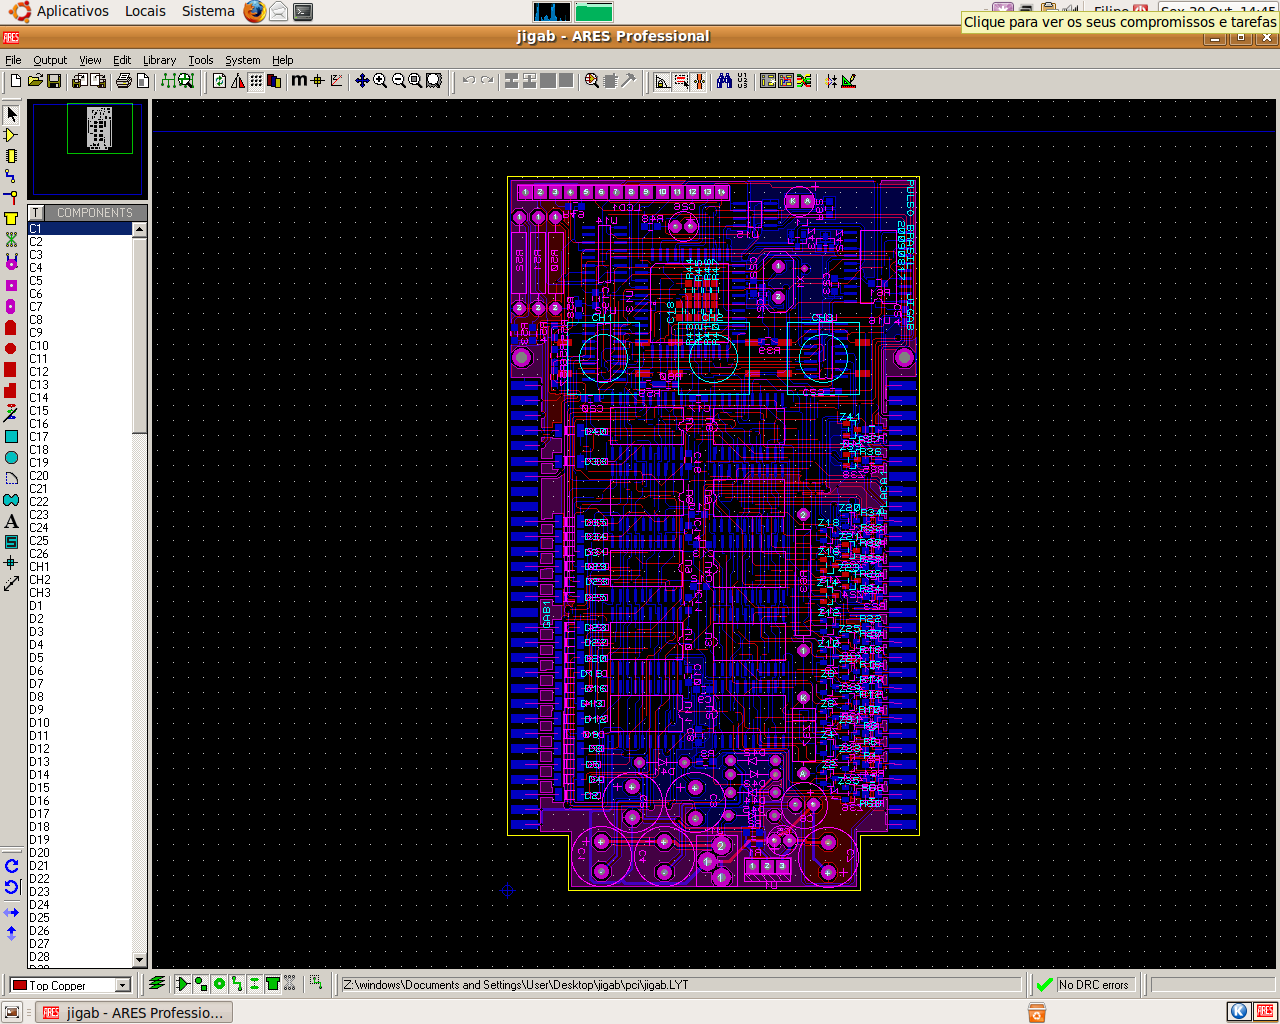
\includegraphics[scale=0.3]{anexo/b1.png}
    \caption{\it Captura de tela do placa roteada no Proteus}
    \label{fig:B1}
\end{figure}

\begin{figure}[htb]
    \centering  % figura centralizada
    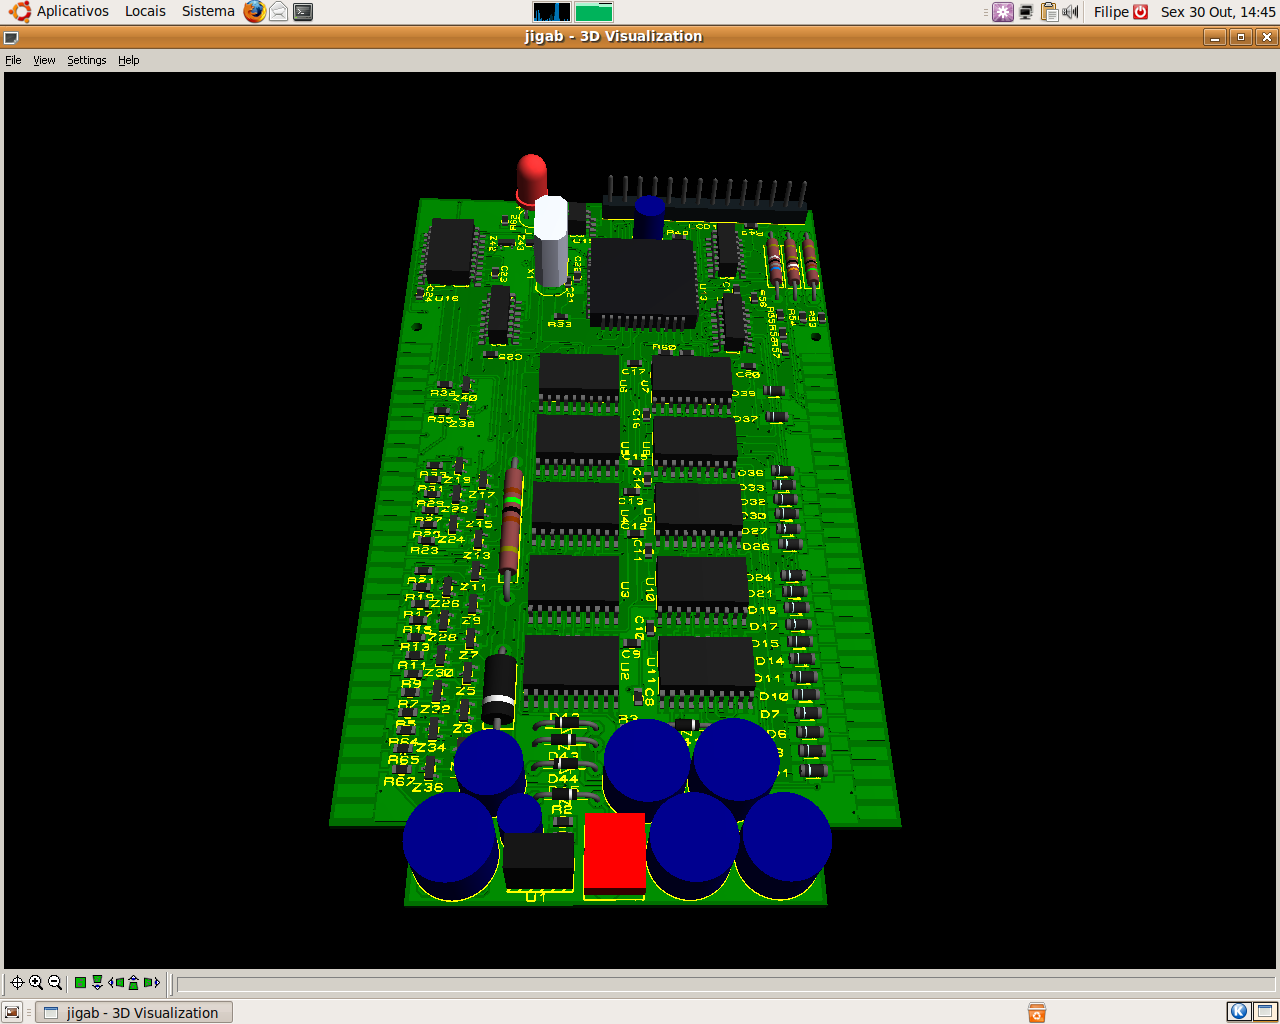
\includegraphics[scale=0.3]{anexo/b2.png}
    \caption{\it Visualiza��o 3D - botton}
    \label{fig:B2}
\end{figure}

\begin{figure}[htb]
    \centering  % figura centralizada
    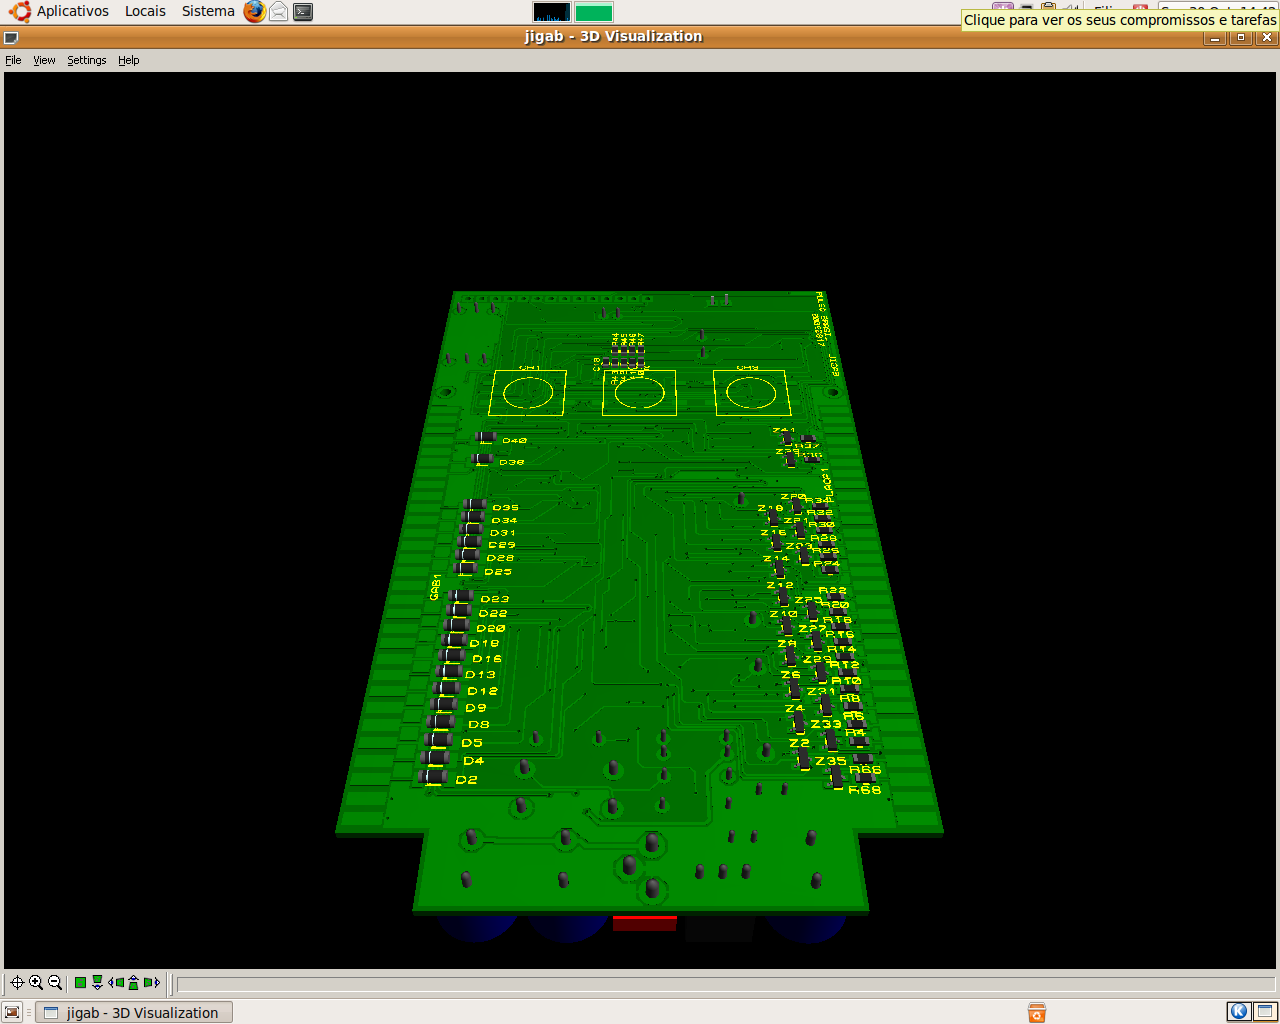
\includegraphics[scale=0.3]{anexo/b3.png}
    \caption{\it Visualiza��o 3D - top}
    \label{fig:B3}
\end{figure}

